% !TeX root = ./00.main.tex
\chapter{Proposta e metodologia}\label{cha:proposta}

\nota{metodologia e implementação}

\begin{resumocap}

  Este Capítulo apresenta a proposta deste trabalho e a metodologia elegida para
  atingir os objetivos.

\end{resumocap}

% Uma Implementação paralela do algoritmo de Detecção de Novidade em Streams MINAS 
\newcommand{\fog}{\emph{fog computing}\xspace}
\newcommand{\cloud}{\emph{cloud computing}\xspace}

\newcommand{\iot}{IoT\xspace}

\newcommand{\stream}{\emph{data stream}\xspace}
\newcommand{\streams}{\emph{data streams}\xspace}
\newcommand{\streamMining}{\emph{data stream mining}\xspace}

\newcommand{\novelty}{\emph{Novelty Detection}\xspace}
\newcommand{\nd}{ND\xspace}
\newcommand{\drift}{\emph{Concept Drift}\xspace}
\newcommand{\evolution}{\emph{Concept Evolution}\xspace}

\newcommand{\mfog}{M-FOG\xspace}
\newcommand{\flink}{\emph{Apache Flink}\xspace}

A Internet das Coisas (\iot) é composta por milhares de dispositivos distribuídos
geograficamente conectados à Internet.
Com capacidades diversas como sensores e atuadores, esses dispositivos produzem e
consomem Fluxos Continuos de Dados (\streams) com diversos objetivos.
Alguns objetivos envolvem a mineração desses fluxos (\streamMining) em busca de
padrões para tomada de decisão e, por vezes requerem também baixa latência.
Para casos de baixa latência ou alta vazão, conexões adequadas para
processamento em nuvem nem sempre são possíveis ou desejáveis, para esses casos
computação em névoa (\fog) é uma solução.

O tema de \streamMining envolve a classificação de novos elementos com base em
um modelo, porém como \streams variam temporalmente e são ilimitados, todas
classes contidas em um \stream não são previamente conhecidas.
A identificação e classificação de novas classes em \streams é denominado
Detecção de Novidades (\novelty, \nd) em \streams.
No tema de \nd, o surgimento e desaparecimento de classes é nomeado Evolução de Conceito
(\evolution) e a mudança no decorrer do \stream é denominado Mudança ou Deriva
de Conceito (\drift).

Além dos aspectos inerentes \streamMining, são considerados na construção de um
sistema que computa \streams a taxa de eventos (itens atômicos de um \stream)
gerados por cada produtor e o número de produtores nesse sistema totalizando o
volume de eventos do sistema.
Volumes elevados são dificilmente computados em apenas um nó e muito menos em um
único núcleo computacional, por esse motivo esses sistemas são distribuídos.

Sistemas que utilizam \nd para \streams gerados por dispositivos \iot devem
utilizar algoritmos que considerem os desafios inerentes de fluxos de dados
(\evolution e \drift) para adequada detecção de novidades e arquiteturas
que atendam os requisitos de volume de mensagens e latência de detecção.
O algoritmo MINAS é adequado pois trata os desafios de \streamMining porém não
tem ainda implementação que atenda os requisitos de volume e latência,
especialmente para aplicações \iot onde um ambiente de \fog é atrativo.

Para preencher a lacuna de algoritmo de \nd em ambiente \fog propõem-se então
\mfog, uma implementação do algoritmo MINAS sobre a plataforma \flink que
considera distribuição em um ambiente de \fog.

% \nota{Reestruturar:
%   A - remember,
%   B - cenário (iot, fog, stream),
%   C - problema (4.1, ND em fog, terminar com minas e cassales),
%   D - solução (4.2, apresetnação, resumo \mfog, metodologia)
% }
% \nota{Falta: fog, processamento distribuído de streams, detecção de novidade}

\section{Descrição da Implementação}\label{sec:descricao}

\newcommand{\source}{\emph{source}\xspace}
\newcommand{\sink}{\emph{sink}\xspace}

\newcommand{\offline}{treinamento\xspace}
\newcommand{\classify}{classificador\xspace}
\newcommand{\detector}{detector\xspace}

\newcommand{\idsiot}{IDSA-IOT\xspace}

Nesta Seção apresenta-se \mfog, objeto proposta deste trabalho.
O \mfog é composto pelos módulos: \offline, \classify e \detector.
Para correta avaliação, \mfog é acompanhado de dois módulos auxiliares:
módulo fonte (\source) e módulo sorvedouro (\sink).

\nota{métodos para alcançar os objetivos}

\nota{o que fazer e como fazer, resultados esperados}

A implementação proposta segue a arquitetura \idsiot proposta por
\citeonline{Cassales2019a}.
A arquitetura \idsiot estabelece que um serviço de captura e tratamento de dados
é instalado na borda de uma rede local com dispositivos \iot.
Na presente implementação
esse serviço de captura e tratamento é representado pelo módulo \source.

\begin{figure}[ht]
  \centering
  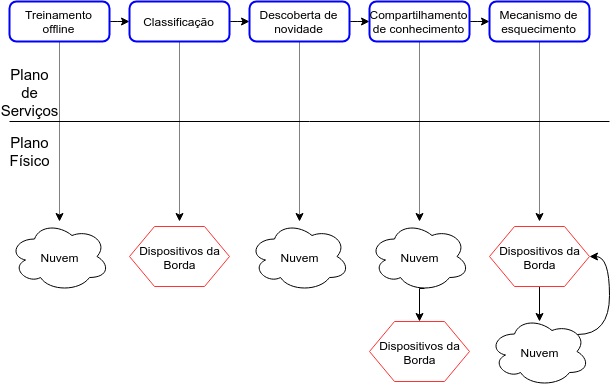
\includegraphics[width=0.8\textwidth]{figuras/cassales-service-physical-pt.png}
  \caption{
    Distribuição de Serviços da Arquitetura \idsiot.
    Produzida e traduzida por \citeonline{Cassales2019a}.
  }
  \label{fig:ids-iot}
\end{figure}

O módulo auxiliar \source é dependente da fonte de dados, executando a transformação dos
formatos dos \datasets para um fluxo de dados compatível com o restante da
implementação.
Além de fornecer dados tratados para \mfog, o módulo \source também fornece
dados para o módulo \sink e \offline.

O módulo auxiliar \sink é responsável por agregar todos resultados do \mfog e,
juntamente com os valores do \dataset fornecidos pelo módulo \source, computar
as métricas de qualidade de classificação e métricas base para as métricas de
escalabilidade e métricas de recursos computacionais.

Os dados resultantes do serviço de captura e tratamento são ingeridos pela
aplicação no módulo \classify por meio de conexão TCP (\emph{Transmission
Control Protocol}) fornecida pela plataforma \flink.
Na plataforma, com o modelo de classificação disponível, os exemplos são
classificados seguindo o algoritmo MINAS original discutido na \refsec{minas-og}.
A etiqueta atribuída pela classificação, ou meta-etiqueta de desconhecido,
juntamente com o exemplo original são enviados para o módulo \sink.
Além disso, se o exemplo não for classificado, o mesmo é enviado para o módulo
\detector.

O módulo \detector é responsável por executar o processo de detecção de
novidade, atualizando o modelo de classificação, e entrega do novo modelo
ao módulo \classify.
Este módulo também envia meta-informações sobre o processo de detecção de
novidade para o módulo \sink.

\section{Metodologia de Avaliação e Resultados Esperados}\label{sec:esperados}

\nota{reestrutura 2:
  A - cenario
  B - metodologia (como, o que vai implementar [kafka, python, flink], como avaliar)
  C - métricas (escalabilidade, qualidade)
  D - resultados preliminares (python/kafka, flink)
}

A avaliação da proposta apresentada será feita por meio de métricas extraídas da
literatura, divididas em duas partes: métricas de qualidade de classificação
e métricas de escalabilidade.

Métricas tradicionais de qualidade de classificação estabelecidas por trabalhos
aprendizado de máquina não são adequadas para avaliar detecção de novidades em
\streams sem tratamento inicial, felizmente o tratamento necessário é
estabelecido por \citeonline{Faria2013} e expandido por
\citeonline{DaSilva2018,DaSilva2018thesis,Costa2019,Costa2019thesis}.
O tratamento estabelece que as métricas são extraídas de uma matriz de erro de
classificação multi-classe \ref{eq:matrix} adaptada para detecção de novidade.
A matriz é preenchida com o número de eventos da classe $c_i$ classificados com
etiqueta $l_j$ até o instante $n$.
A equação \ref{eq:classes} representa o conjunto de classes presentes nos eventos
do fluxo até o instante $n$ e a equação \ref{eq:labels} representa o conjunto
de etiquetas atribuídas pelo classificador à eventos até o mesmo instante.

\begin{align}
  % x_n &= classify_{n-1}(x_n)\\
  % e_{i, j} &= classify_{n-1}(x_n)\\
  \mathbf{C}_n &= \{ c_1, c_2, \cdots, c_M \}  \label{eq:classes} \\
  \mathbf{L}_n &= \{ l_1, l_2, \cdots, l_J \}  \label{eq:labels} \\
  \mathbf{E}_n &= \begin{pmatrix}
    e_{1,1} & e_{1,2} & \cdots & e_{1,J} \\
    e_{2,1} & e_{2,2} & \cdots & e_{2,J} \\
    \vdots  & \vdots  & \ddots & \vdots  \\
    e_{M,1} & e_{M,2} & \cdots & e_{M,J} 
  \end{pmatrix}  \label{eq:matrix}
\end{align}

As métricas selecionadas são taxa de desconhecidos ($UnkR$) \cite{Faria2013},
acurácia média ($acc$) e Macro F-score ($Fscore$, F1M)
\cite{Sokolova2009,DaSilva2018thesis}.

% e \emph{Logarithm Loss} ($\mathcal{L}$).

%   \mathbf{C} &= [c_1, c_2, \cdots, c_I] \\
%   \mathbf{L} &= [l_1, l_2, \cdots, l_J] \\
%   \forall n\to\infty: & \\
%   \mathbf{C}_{n}  &= \mathbf{C}_{n-1} \cup c \in \mathbf{C} \\
%   \mathbf{L}_{n}  &= \mathbf{L}_{n-1} \cup l \in \mathbf{L} \\
%   X               &= (n, \overrightarrow{x}, c) \\
%   Y = \mathrm{classifica}(X) &= (n, \overrightarrow{x}, l \vee \text{unk}) \\
%   \mathbf{Unk}    &= \{ Y : (_, _, l = \text{unk}) \} \\
% \mathit{UnkR}_n   &= \frac{ \#Unk }{n}

\begin{align}
  \mathit{UnkR}       &= \frac{1}{M} \sum_{i=1}^{M} \frac{\#Unk_i}{\#ExC_i}\\
  \mathit{acc}        &= \frac{1}{M} \sum_{i=1}^{M} \frac{tp_i + tn_i}{tp_i+fn_i+fp_i+tn_i}
  = \frac{1}{M} \sum_{i=1}^{M} \frac{\#Acc_i}{\#ExC_i}\\
  \mathit{Precision}  &= \frac{1}{M} \sum_{i=1}^{M} \frac{tp_i}{tp_i+fp_i} \\
  \mathit{Recall}     &= \frac{1}{M} \sum_{i=1}^{M} \frac{tp_i}{tp_i+fn_i} \\
  \mathit{Fscore}_\beta &= (\beta^2 +1) \cdot
  \frac{
  \mathit{Precision} \cdot \mathit{Recall}
  }{
    \beta^2 \cdot \mathit{Precision} +\mathit{Recall}
  }\\
  \mathit{Fscore}_1   &= 2 \cdot \frac{
    \mathit{Precision} \cdot \mathit{Recall}
    }{
      \mathit{Precision} +\mathit{Recall}
    } 
\end{align}
% = 2 \cdot \frac{tp}{2 \cdot tp + fn + fp}
% \mathcal{L}         &= \frac{-1}{N} \sum_{i=1}^{M} \sum_{j=1}^{J} y_{i,j} \log(p_{i,j})

O tratamento do fluxo de saída é realizado no módulo \sink onde tem-se
disponível o fluxo original com as etiquetas corretas.
Esse módulo deve levar em consideração que
como pode haver reclassificação de um evento, previamente rotulado como
desconhecido, em padrões oriundos de classe novidade ou extensão devido ao
processo de detecção de novidades executado posteriormente ao surgimento
do padrão em questão.
Portanto os resultados são computados em função do fluxo de saída, então $n$ nas
equações são o índice do evento de saída.
$\mathbf{unk}$ é o conjunto de eventos marcados como desconhecidos.

% \begin{align}
%   E_{n,i,j} &= \bordermatrix{~ & c_i & \neg c_i \cr
%   l_j       & TP = \alpha           & FP = \gamma - \alpha                 \cr
%   \neg l_j  & FN = \beta - \alpha   & TN = n - (\alpha + \beta + \gamma)  \cr} \\
%   FM1       &= \frac{TP}{TP+\frac{FP+FN}{2}}
% \end{align}

% Os valores da matriz de erro para 

% \begin{align}
%   \alpha _j &= max( \{ |e_{i,j}|: i = 1 .. I \wedge \in \mathbf{E}_n \})
%           & \text{máximo da linha (etiqueta)} \\
%   a_j &= i: |e_{i,j}| = \alpha _j
%           & \text{índice da classe associada à etiqueta} \\
%   \beta   &= \sum_{j = 0}^{J} e_{i,j} : e_{i,j} \in \mathbf{E}_n
%           & \text{soma de uma coluna (etiqueta)} \\
%   \gamma  &= \sum_{i = 0}^{I} a_{i,j} : e_{i,j} \in \mathbf{E}_n
%           & \text{soma de uma linha (classe)}
% \end{align}

As métricas de escalabilidade selecionadas são número de nós processadores, tipo
de processadores, uso de memória, tempo de processamento, taxa de eventos
processados e latência entre a produção e classificação de um evento.

Da implementação \mfog é prevista execução de experimentos com \datasets
diversos, em especial os \datasets reais que contém evolução de conceitos.
Os resultados desses experimentos são válidos se contém as seguintes métricas
para o \mfog: \begin{enumerate*}[label={\alph*)}]
  \item qualidade de classificação (taxa de desconhecidos, F1M)
  \item escalabilidade (número de processadores, volume processado, tempo decorrido)
  \item recursos computacionais utilizados (memória, tempo de processamento, operações de leitura e escrita)
\end{enumerate*}
e para o minas somente as métricas de qualidade de classificação.

% O foco da revisão da literatura acadêmica é em trabalhos que abordem:
% processamento de fluxos de dados, classificação de fluxo de dados, detecção de
% novidades em fluxo de dados e processamento e distribuído de fluxo de dados.
% O objetivo da revisão é o estabelecimento do estado da arte desses assuntos
% e para que alguns desses trabalhos sirvam para comparações e relacionamentos.
% Além disso, desses trabalhos extrai-se métricas de qualidade de classificação
% (por exemplo taxa de falso positivo e matriz de confusão) e métricas de
% escalabilidade (taxa de mensagens por segundo e escalabilidade vertical ou
% horizontal).

% A revisão da literatura técnica foca em plataformas, ferramentas e técnicas
% para realizar a implementação proposta.
% Portanto, serão selecionadas plataformas de processamento distribuído de fluxos
% contínuos de dados e técnicas de aprendizado de máquina associadas a elas. Dessa revisão também são obtidas
% as técnicas ou ferramentas necessárias
% para extração das métricas de avaliação bem como \emph{data sets}
% públicos relevantes para detecção de novidades em DS.

% Uma vez definidos o estado da arte, as ferramentas técnicas e os
% \emph{data sets}, o passo seguinte é a experimentação.
% Nesse passo é desenvolvida uma aplicação multi-processada que, com base no
% algoritmo MINAS \cite{Faria2016minas}, classifica e detecta novidades em DS.
% Os resultados de classificação dessa implementação equivalem-se aos resultados 
% de classificação da implementação original, validando assim essa nova
% aplicação. 

% Além disso, experimentos com a implementação e variações em \emph{data sets} e
% cenários de distribuição em \emph{fog} coletando as métricas de classificação e escalabilidade.
% Os resultados serão comparados entre si e com outros trabalhos.

% E ao final, a aplicação, resultados, comparações e discussões serão publicados
% nos meios e formatos adequados como repositórios técnicos, eventos ou revistas
% acadêmicas.

% meh
% \section{Descrição do \mfog}

% Esta \Section descreve 

% Esse Capítulo apresenta-se a descrição de uma implementação paralela do algoritmo
% de detecção de novidades em fluxos de dados contínuos (\emph{Novelty Detection
% in Data Streams}) MINAS inserido no cenário de processamento distribuído no
% ambiente de computação em névoa (\fog) com ênfase nos fluxos gerados por
% dispositivos de Internet das Coisas (\iot) doravante referido por \mfog ou 
% ``a presente implementação''.
% Os requisitos dessa implementação são derivados das lacuna discutidas no
% \refcap{related}.

% \nota{resumo e retomada do objetivo}


% Uma das lacunas é a falta de uma implementação do algoritmo
% MINAS mais próxima de aplicações reais, ou seja:
% que trate de fluxos realistas em contraste aos conjuntos de dados (\datasets)
% sintéticos;
% que considere restrições computacionais tanto teóricas que são características
% de processamento de fluxos contínuos e ilimitados como restrições práticas
% de ambientes diversos como computação pessoal (\emph{Desktop Computing}), 
% computação em nuvem (\cloud) e computação em névoa (\fog).

% Outras lacunas são encontrada na implementação de sistemas de que dependem de
% algoritmos de detecção de novidades. Nessas implementações nota-se a falta de
% algoritmos que tenham as considerações teóricas inerentes da variabilidade de
% dados em fluxos contínuos de dados como deriva e evolução de conceito (\drift e
% \evolution).
% Por outro lado, outros sistemas consideram a variabilidade porém o
% mecanismo de atualização do modelo assume que as etiquetas reais estarão
% disponíveis após classificação (\emph{feedback}) imediatamente ou com atraso
% predizível.
% A suposição de \emph{feedback} em fluxos reais também não é realista pois
% a presença de um especialista que classifique corretamente os exemplos
% solicitados é, na melhor das hipóteses, eventual e não contínua contrastando com
% a natureza do fluxo de dados.

% % Para cumprir os objetivos citados na \refsec{objetivos}, foi identificado a necessidade
% % de um processo exploratório seguido de experimentação. Tal processo inclui a
% % revisão da literatura, tanto acadêmica quanto técnica, seguida da experimentação
% % através de implementação de aplicação e testes.

% \section{Cenário}\label{sec:cenario}

% A presente Seção descreve o cenário base para a proposta de implementação,
% expondo características, desafios e hipóteses que a implementação deve atender.

% A Internet das Coisas \iot é composta por milhares de dispositivos distribuídos
% geograficamente conectados à Internet.
% Com capacidades diversas como sensores e atuadores, esses dispositivos dependem
% de conexões para executarem suas funções, enviando e recebendo informações
% trocadas com outros dispositivos ou aplicações centrais hospedadas em ambiente
% \cloud.
% A a dependência de comunicação é uma restrição que tem diversas implicações
% como confiabilidade de um sistema e, dependendo da conexão limita ou impede
% funcionalidades comuns em outros ambientes.
% Além das restrições, devido aos encargos atribuídos à manutenção da comunicação,
% o envio e recebimento de dados em dispositivos deve ser minimizado.

% % estou deixando implícito as restrições como baterias :(

% Mesmo com as restrições e desafios, a implementação de dispositivos ainda é
% vantajosa, pois o valor sobrepõe o custo.
% Esse valor origina de várias fontes como automação, redução de risco e coleta
% de dados granulares que possibilitam análises antes impraticáveis.
% A coleta de dados para análise contínua é um dos principais fatores na
% implantação de um sistema IoT levando a geração de diversos fluxos com
% propriedades e processos igualmente diversos.
% % A análise constante de dados 